\chapter{Antecedentes}
\labch{antec}
\section{pH}
\labsec{ph}
Una estrategia nueva, investigada en la tesis de maestría del presente autor%\sidenote{Disponible en el siguiente enlace \url{https://github.com/murpholinox/tesis\_maestria}}
, fue modificar el pH dentro de los cristales macromoleculares. Esta idea se basa en la idea general de los radioprotectores y se detalla a continuación. 

La radiólisis del agua produce las siguientes reacciones \sidecite{VonSonntag2006}:
\begin{align}
	\ce{H2O           &->[rayos X]     H2O^{.+}    +             e^{-}}  \\
	\ce{H2O           &->[rayos X]     H2O^{*}}                          \\
	\ce{H2O^{.+}      &->  \color{red}HO^{.}       +              H^{+}} \\
	\ce{e^{-} + nH2O  &->  \color{red}e^{-}_{solv.}}                     \\
	\ce{H2O^{*}       &->  \color{red}HO^{.}       +   \color{red}H^{.}}
\end{align} 
Donde las especies químicas denotadas en rojo, representan los primeros radicales libres presentes en un cristal macromolecular (el radical hidroxilo, el electrón solvatado y el radical hidrógeno).% Esto es relevante porque en general el contenido de solvente, agua, en un cristal macromolecular es bastante. 

Con la criocristalografía de rayos X, se impide la difusión del radical hidroxilo \sidecite{Owen2012a}. Sin embargo, el \ce{e^{-}_{solv.}} y el radical hidrógeno todavía son móviles. El electrón solvatado puede moverse del solvente a la proteína, donde es capaz de viajar a través de la cadena polipeptídica hasta hallar un centro electrofílico, como por ejemplo átomos metálicos o puentes disulfuro (\reffig{fig:symons92}) \sidecite{Symons1997}. Se ha propuesto que esta es la razón del origen del orden en el que se manifiesta el daño por radiación específico, pues la captura de electrones es mucho más específica que la captura de huecos positivos \sidecite{Close2019}. 

\begin{figure}[h]
	\centering
	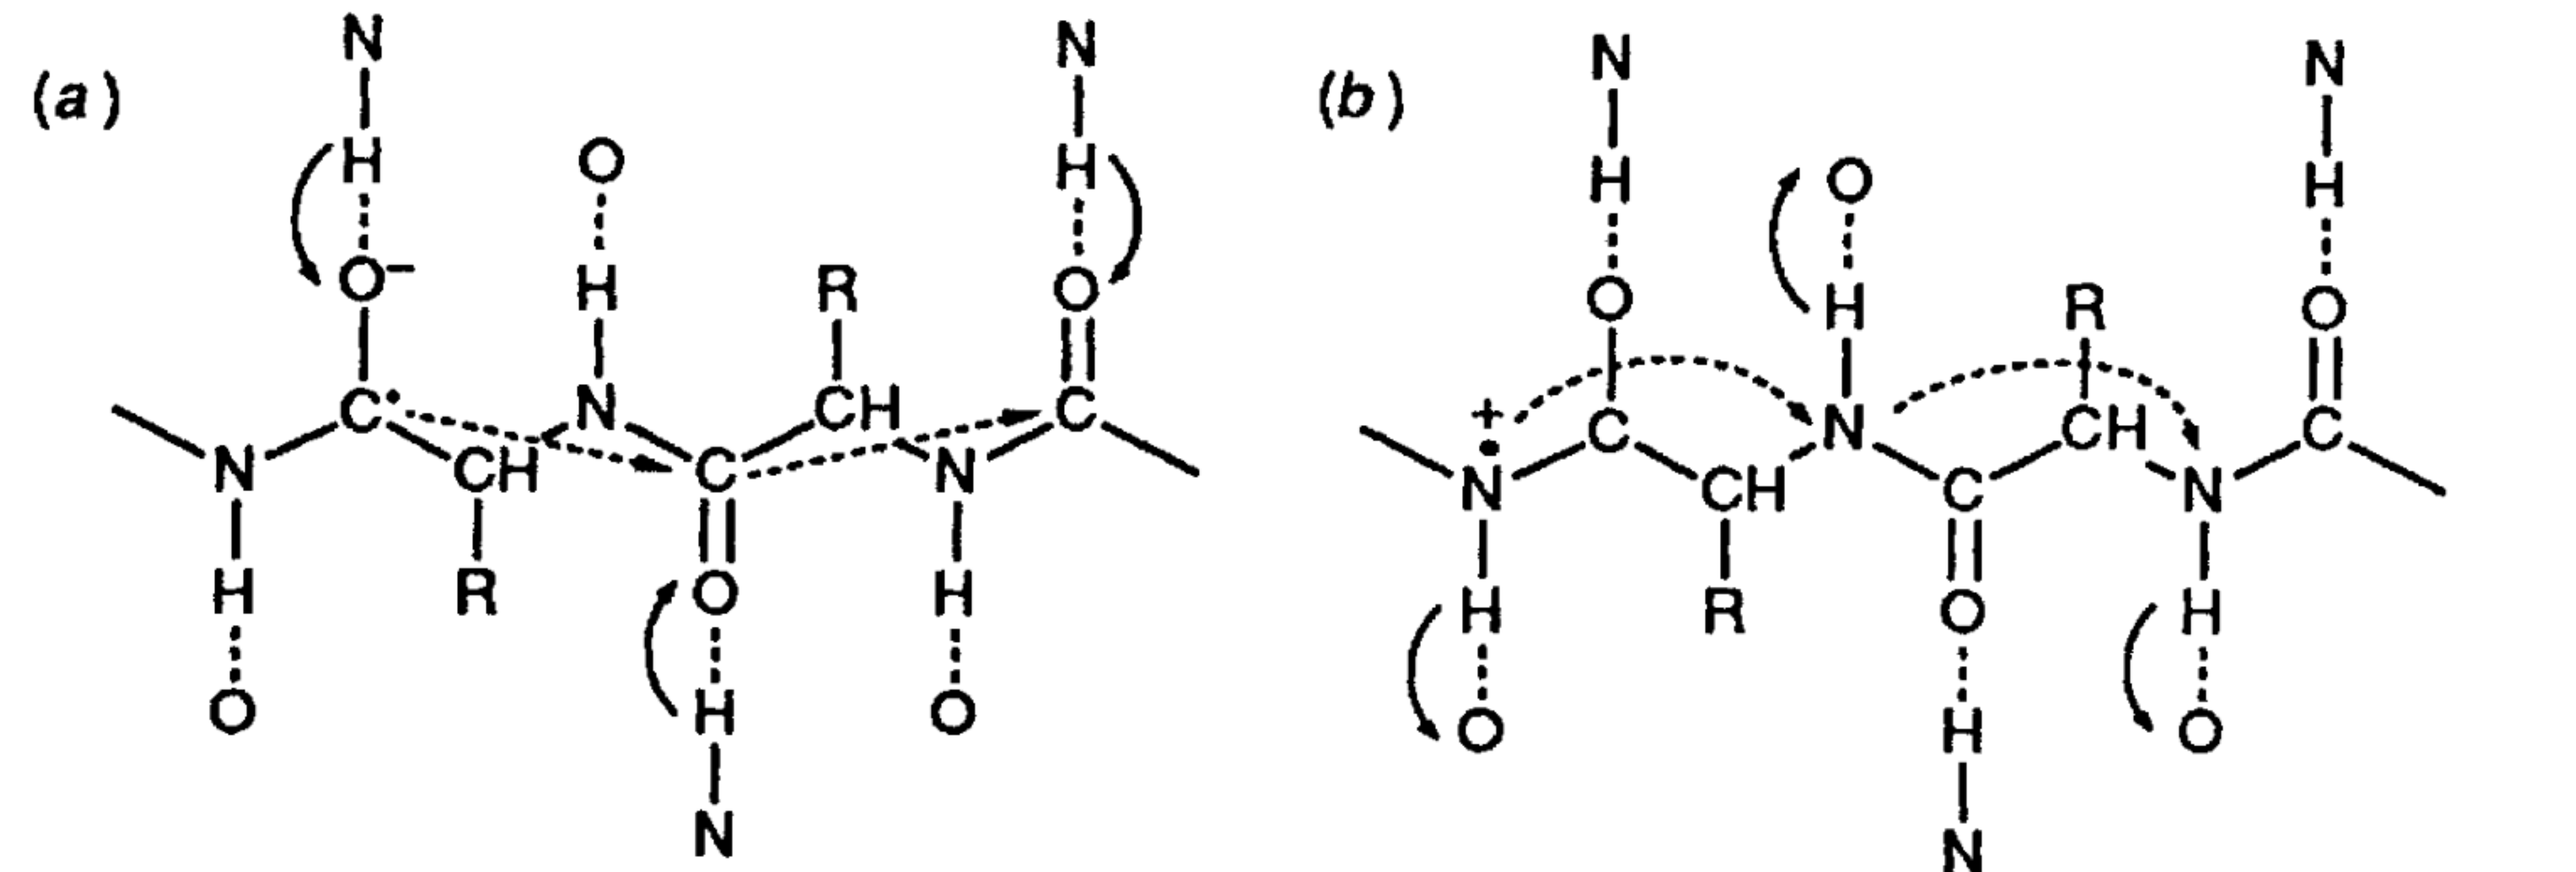
\includegraphics[width=0.9\textwidth]{imgs/symons92.png}
	\caption[Movimiento de cargas en la cadena polipeptídica]{Moviento de electrones (a) y huecos positivos (b), a través de la cadena polipeptídica. Fuente: \cite{Symons1997}.}
	\labfig{fig:symons92}
\end{figure}

Por su parte, el radical hidrógeno sigue una reacción de recombinación formando como producto final \ce{H2}, propuesto como el responsable directo del daño por radiación global \sidecite{Meents2010}.

La idea de ocupar al protón como radioprotector dentro del cristal macromolecular, se basa en que el electrón solvatado y el átomo de hidrógeno se encuentran en un equilibrio ácido-base; por lo que el electrón solvatado se convierte en \ce{H^{.}} en una solución ácida. %De hecho, en el campo de la química de las radiaciones, es común estudiar el efecto de un radical al convertir los otros radicales en especies el radical estudiado. 
\begin{equation}
\ce{e^{-}_{solv.} + H^{+} <=> H^{.}}
\end{equation}

En la tesis de maestría se usó como sistema de estudio la lisozima de clara de huevo de gallina, que presenta cuatro puentes disulfuro. La idea era que el ion hidronio, también conocido como oxidanio, funcionara como radioprotector al interactuar con los electrones solvatados antes que estos interactuaran con los puentes disulfuro de esta proteína. Para esto, se comparó el daño específico sobre los puentes disulfuro en cristales de lisozima a tres niveles de pH: \num{3.7}, \num{4.7} y \num{5.7}. Los resultados obtenidos fueron opuestos a los esperados: a niveles comparables de dosis de radiación absorbida, el cristal con el pH más ácido presentó mayor daño por radiación que el cristal con el pH más básico.

La variabilidad entre cristales macromoleculares, aún proveniendo de la misma condición de cristalización, puede llevar a conclusiones erróneas \sidecite{Nowak2009}. En la tesis de maestría no se pudo concluir si la diferencia observada era estadísticamente significativa, pues no se realizaron las repeticiones necesarias para cada condición experimental.


